% 
% Annual Cognitive Science Conference
% Sample LaTeX Paper -- Proceedings Format
% 

% Original : Ashwin Ram (ashwin@cc.gatech.edu)       04/01/1994
% Modified : Johanna Moore (jmoore@cs.pitt.edu)      03/17/1995
% Modified : David Noelle (noelle@ucsd.edu)          03/15/1996
% Modified : Pat Langley (langley@cs.stanford.edu)   01/26/1997
% Latex2e corrections by Ramin Charles Nakisa        01/28/1997 
% Modified : Tina Eliassi-Rad (eliassi@cs.wisc.edu)  01/31/1998
% Modified : Trisha Yannuzzi (trisha@ircs.upenn.edu) 12/28/1999 (in process)
% Modified : Mary Ellen Foster (M.E.Foster@ed.ac.uk) 12/11/2000
% Modified : Ken Forbus                              01/23/2004
% Modified : Eli M. Silk (esilk@pitt.edu)            05/24/2005
% Modified : Niels Taatgen (taatgen@cmu.edu)         10/24/2006
% Modified : David Noelle (dnoelle@ucmerced.edu)     11/19/2014

%% Change "letterpaper" in the following line to "a4paper" if you must.

\documentclass[10pt,letterpaper]{article}

\usepackage{cogsci}
\usepackage{pslatex}
\usepackage{apacite}
\usepackage{graphicx}



\title{[Cute title]: The Pragmatics of Spatial Language}
 
%\author{{\large \bf Morton Ann Gernsbacher (MAG@Macc.Wisc.Edu)} \\
%  Department of Psychology, 1202 W. Johnson Street \\
%  Madison, WI 53706 USA
%  \AND {\large \bf Sharon J.~Derry (SDJ@Macc.Wisc.Edu)} \\
%  Department of Educational Psychology, 1025 W. Johnson Street \\
%  Madison, WI 53706 USA}

\author{
{\large \bf Author 1 (email@place.edu)} \\
  Department of Psychology, University of Gondor\\
  \And{\large \bf Author 2 (email@place.edu)} \\
  Department of Cognitive Science, University of Mordor \\
  \\
 \AND{\large \bf Author 3 (email@people.edu)} \\
  Department of Computer Science, University of Shire\\
}

\begin{document}
\maketitle

\begin{abstract}
People use spatial language

\textbf{Keywords:} 
Pragmatics, implicature, spatial language
\end{abstract}

\section{Introduction}

he spatial world is rich and complex, but our spatial vocabulary is often coarse and limited. For example, English---like many other languages---has a restricted and closed class of spatial prepositions~\cite{talmy83,talmy00,landau93} such as ``in,'' ``on,'' and ``near'' that describe a potentially infinite set of spatial relations. This raises a natural question: How do we make accurate inference in spatial situations when our spatial vocabulary is somewhat impoverished?

A plausible solution to this question is via pragmatics~\cite{grice75,horn84}. On this view, listener would make inferences that go beyond the literal meaning of speaker's utterance by taking speaker's perspective in a given context. After all, inference is cheap and articulation is expensive~\cite{levinson00}, and therefore we expect pragmatics to play a key role in enriching the core spatial vocabulary that can be limited under many different situations. 

To illustrate this idea, we describe a simple scenario that provides the basis of our study. Figure~\ref{illustration} shows the map of a small city with two quarters (i.e. represented by the red and blue rectangles respectively) and a plaza (i.e. represented by the dashed circle), where the plaza is located inside the red quarter. Suppose you were told that ``a gold lily grew in the red quarter.'' Where would you think the flower had grown on the map? There are two possiblilities. In the first case, a listener who takes the literal meaning of ``in'' would infer the lily to have grown anywhere within the red square. This follows from the fact that the core meaning of ``in'' would simply refer to locations within the enclosure of the red rectangle as bounded by its sides. However, a more sophisticated listener might instead reason as follows for a more precise spatial inference: ``If the lily had grown in the plaza, the speaker would have said that the lily grew in the plaza. However, given that she didn't say so, the lily must have grown within the red quarter but in areas excluding that plaza.'' Thus, this pragmatic listener would be able to make a more specific prediction than the literal listener about where the lily might have grown, even though the speaker's utterance is identical in both cases. In this respect, pragmatic reasoning helps the listener to locate things beyond the precision of what the meaning of ``in'' conventionally renders by combining perspective taking (i.e. playing the role of speaker) with one's knowledge of the spatial situation (i.e. the fact that the plaza is located inside the red square).

\begin{figure}[h]
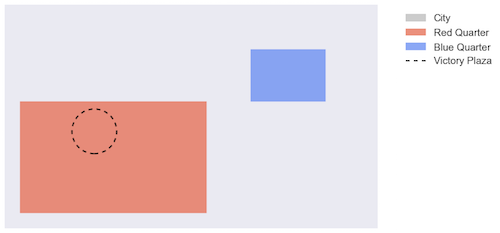
\includegraphics[scale=.5]{figures/cityA1.png}
\caption{Illustration of a simple spatial situation.}
\label{illustration}
\end{figure}

In this study, we explore the relation between pragmatics and spatial language using probabilistic programs~\cite{}. MAYBE NOAH CAN SAY SOMETHING HERE? Previous work has discussed the role of pragmatics in spatial locative expressions~\cite{herskovits85,herskovits87}. However, to our knowledge, formal work in this domain is scarce. Moreover, recent computational studies have emphasized speaker's role in the pragmatic use of spatial language~\cite{carstensen14,golland10}, but not how listener makes pragmatic inference based on implicatures. We seek to bridge this gap with a formal model that makes quantitative predictions about listener's behavior as guided by spatial language and pragmatics. 

To preview our results ... MAYBE TOMER CAN FILL IN THE EXCITING RESULTS PREVIEW HERE?



\section{Modeling spatial implicature}\label{mod}

Let's model it!

\section{Experiment}\label{sec:exps}

We examined people's spatial inferences and the predictions of our model regarding the spatial terms `in' and `near'. We put participants in the role of a listener and asked them to guess where an event happened on a map, based on the utterance of a speaker who had access to the location of the event. 

\subsection{Participants, materials and methods}

Participants ($N=49$, 13 female, median age 29) were recruited through Amazon's Mechanical Turk service. 

We constructed 4 simple city maps (see Fig. XX), each containing 2 ``Quarters'' of different size and color, and a circle marked as ``Victory Plaza''. The location of Victory Plaza varied among the 4 cities, while the location of the Quarters remained the same. To broadly control for effects of color and position, we created another set of 4 maps by flipping the original maps along the vertical and horizontal axis, and changing the color of the quarters, making 8 maps in total. Participants were randomly assigned to one of the two map groups. 

Participants were shown an example map and were informed that throughout the experiment they would see similar maps. Participants were told that anywhere in the city they're shown, a special flower called a `Gold Lily' can grow, and that their task is to find the Gold Lilies. 

Participants were further told that in their task a person will tell them where a Gold Lily grew, and that this person can say the Gold Lily grew \textit{in} a location or \textit{near} a location. This person was also said to be reasonable, and honest. As an example, a participant might read the sentence `A person tells you: A Gold Lily grew in the Red Quarter'. Participants made their guess by clicking directly on the maps they were shown.

For each of the 4 maps in their group, participants were prompted with a sentence made of $word \times location$ combinations, where $word \in [In,\ Near]$ and $location \in [Red\ Quarter,\ Blue\ Quarter,\ Victory\ Plaza,\ City]$. We chose not to include the combination ``Near the City'', as this area was not in the scope of the image and likely to create confusion. In total, each participant was prompted with 28 different sentences, shown in random order. 

\subsection{Results} 

\begin{figure*}[t]
\begin{center}
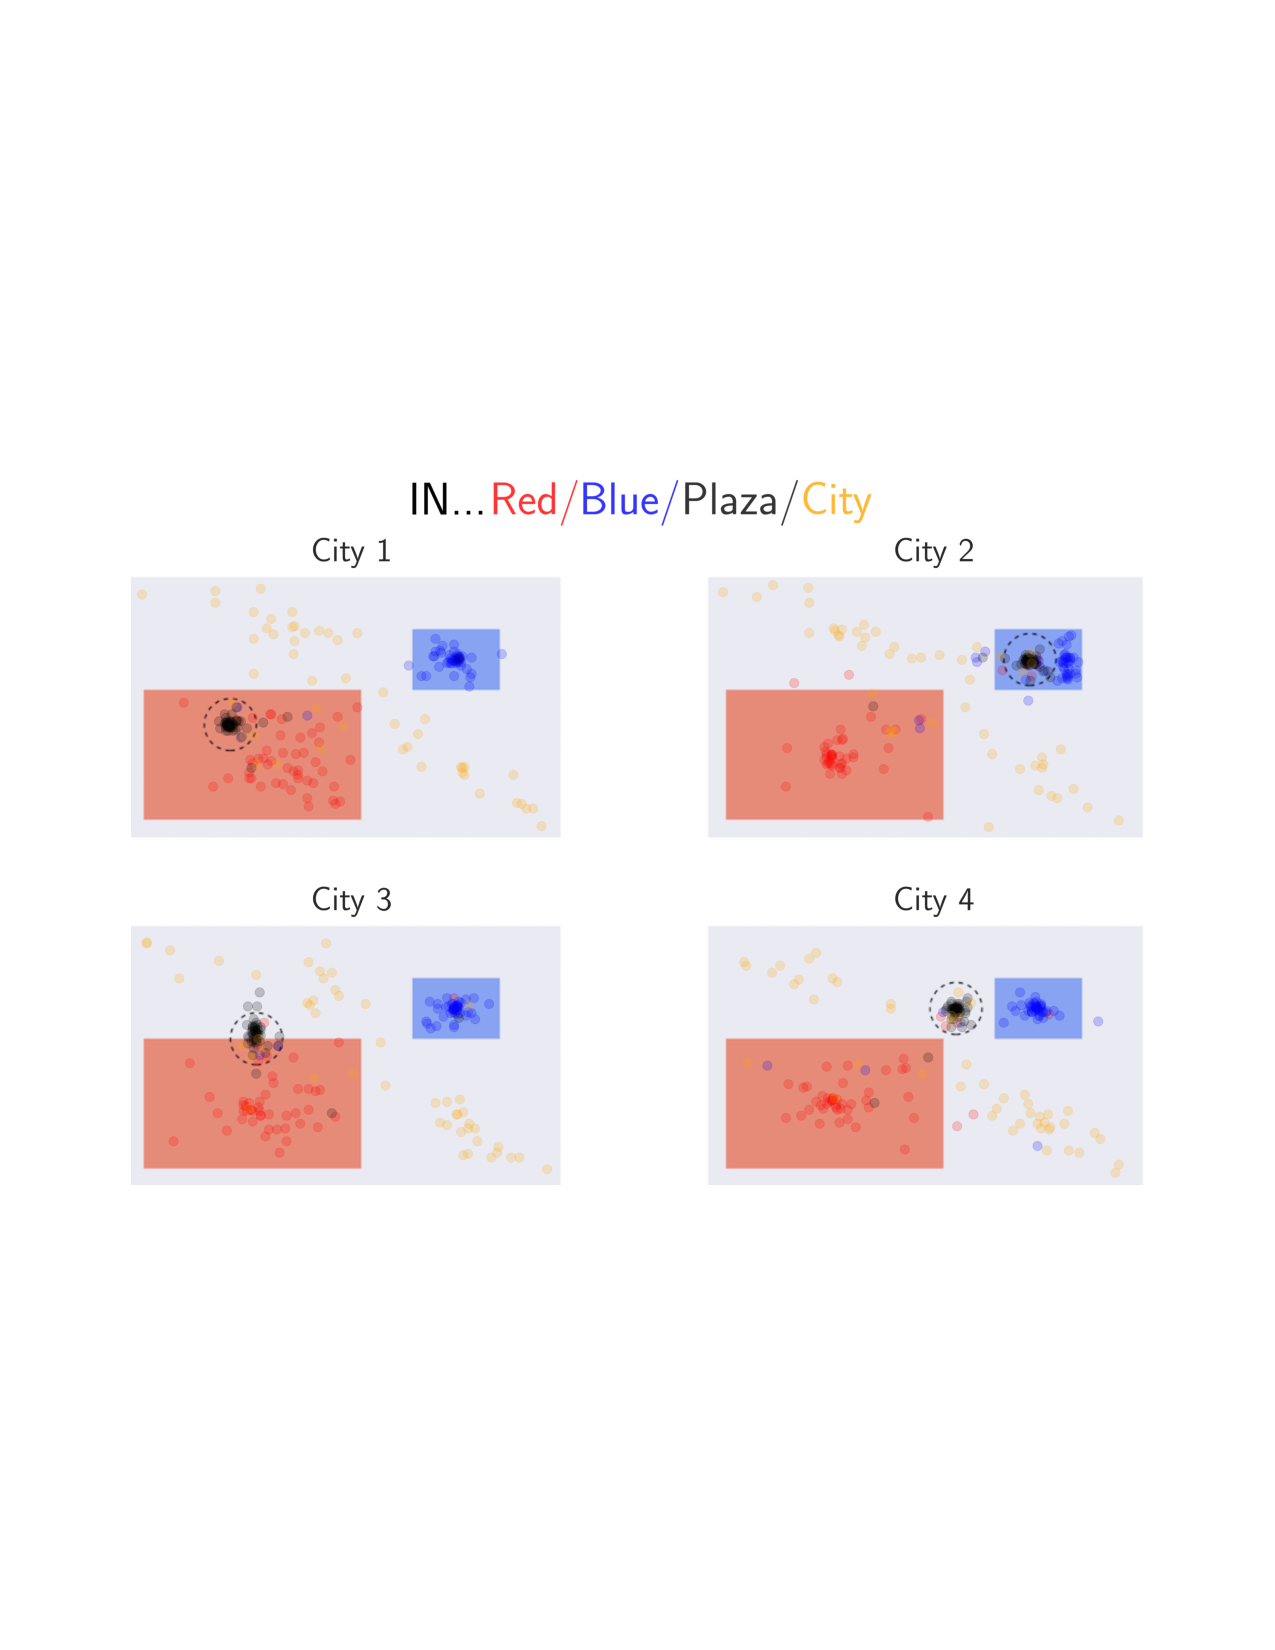
\includegraphics[width=\textwidth]{figures/In.pdf}
\end{center}
\caption{This is a figure.} 
\label{sample-figure}
\end{figure*}








\section{Acknowledgments}


\section{References Instructions}

Follow the APA Publication Manual for citation format, both within the
text and in the reference list, with the following exceptions: (a) do
not cite the page numbers of any book, including chapters in edited
volumes; (b) use the same format for unpublished references as for
published ones. Alphabetize references by the surnames of the authors,
with single author entries preceding multiple author entries. Order
references by the same authors by the year of publication, with the
earliest first.

Use a first level section heading, ``{\bf References}'', as shown
below. Use a hanging indent style, with the first line of the
reference flush against the left margin and subsequent lines indented
by 1/8~inch. Below are example references for a conference paper, book
chapter, journal article, dissertation, book, technical report, and
edited volume, respectively.

\nocite{ChalnickBillman1988a}
\nocite{Feigenbaum1963a}
\nocite{Hill1983a}
\nocite{OhlssonLangley1985a}
% \nocite{Lewis1978a}
\nocite{Matlock2001}
\nocite{NewellSimon1972a}
\nocite{ShragerLangley1990a}


\bibliographystyle{apacite}

\setlength{\bibleftmargin}{.125in}
\setlength{\bibindent}{-\bibleftmargin}

\bibliography{CogSci_Template}


\end{document}
